\documentclass[]{article}
\usepackage{lmodern}
\usepackage{amssymb,amsmath}
\usepackage{ifxetex,ifluatex}
\usepackage{fixltx2e} % provides \textsubscript
\ifnum 0\ifxetex 1\fi\ifluatex 1\fi=0 % if pdftex
  \usepackage[T1]{fontenc}
  \usepackage[utf8]{inputenc}
\else % if luatex or xelatex
  \ifxetex
    \usepackage{mathspec}
  \else
    \usepackage{fontspec}
  \fi
  \defaultfontfeatures{Ligatures=TeX,Scale=MatchLowercase}
\fi
% use upquote if available, for straight quotes in verbatim environments
\IfFileExists{upquote.sty}{\usepackage{upquote}}{}
% use microtype if available
\IfFileExists{microtype.sty}{%
\usepackage{microtype}
\UseMicrotypeSet[protrusion]{basicmath} % disable protrusion for tt fonts
}{}
\usepackage[margin=1in]{geometry}
\usepackage{hyperref}
\hypersetup{unicode=true,
            pdftitle={Urban ecological corridors in Ouro Preto: removing STs from corridors},
            pdfauthor={Bernardo Niebuhr},
            pdfborder={0 0 0},
            breaklinks=true}
\urlstyle{same}  % don't use monospace font for urls
\usepackage{color}
\usepackage{fancyvrb}
\newcommand{\VerbBar}{|}
\newcommand{\VERB}{\Verb[commandchars=\\\{\}]}
\DefineVerbatimEnvironment{Highlighting}{Verbatim}{commandchars=\\\{\}}
% Add ',fontsize=\small' for more characters per line
\usepackage{framed}
\definecolor{shadecolor}{RGB}{248,248,248}
\newenvironment{Shaded}{\begin{snugshade}}{\end{snugshade}}
\newcommand{\AlertTok}[1]{\textcolor[rgb]{0.94,0.16,0.16}{#1}}
\newcommand{\AnnotationTok}[1]{\textcolor[rgb]{0.56,0.35,0.01}{\textbf{\textit{#1}}}}
\newcommand{\AttributeTok}[1]{\textcolor[rgb]{0.77,0.63,0.00}{#1}}
\newcommand{\BaseNTok}[1]{\textcolor[rgb]{0.00,0.00,0.81}{#1}}
\newcommand{\BuiltInTok}[1]{#1}
\newcommand{\CharTok}[1]{\textcolor[rgb]{0.31,0.60,0.02}{#1}}
\newcommand{\CommentTok}[1]{\textcolor[rgb]{0.56,0.35,0.01}{\textit{#1}}}
\newcommand{\CommentVarTok}[1]{\textcolor[rgb]{0.56,0.35,0.01}{\textbf{\textit{#1}}}}
\newcommand{\ConstantTok}[1]{\textcolor[rgb]{0.00,0.00,0.00}{#1}}
\newcommand{\ControlFlowTok}[1]{\textcolor[rgb]{0.13,0.29,0.53}{\textbf{#1}}}
\newcommand{\DataTypeTok}[1]{\textcolor[rgb]{0.13,0.29,0.53}{#1}}
\newcommand{\DecValTok}[1]{\textcolor[rgb]{0.00,0.00,0.81}{#1}}
\newcommand{\DocumentationTok}[1]{\textcolor[rgb]{0.56,0.35,0.01}{\textbf{\textit{#1}}}}
\newcommand{\ErrorTok}[1]{\textcolor[rgb]{0.64,0.00,0.00}{\textbf{#1}}}
\newcommand{\ExtensionTok}[1]{#1}
\newcommand{\FloatTok}[1]{\textcolor[rgb]{0.00,0.00,0.81}{#1}}
\newcommand{\FunctionTok}[1]{\textcolor[rgb]{0.00,0.00,0.00}{#1}}
\newcommand{\ImportTok}[1]{#1}
\newcommand{\InformationTok}[1]{\textcolor[rgb]{0.56,0.35,0.01}{\textbf{\textit{#1}}}}
\newcommand{\KeywordTok}[1]{\textcolor[rgb]{0.13,0.29,0.53}{\textbf{#1}}}
\newcommand{\NormalTok}[1]{#1}
\newcommand{\OperatorTok}[1]{\textcolor[rgb]{0.81,0.36,0.00}{\textbf{#1}}}
\newcommand{\OtherTok}[1]{\textcolor[rgb]{0.56,0.35,0.01}{#1}}
\newcommand{\PreprocessorTok}[1]{\textcolor[rgb]{0.56,0.35,0.01}{\textit{#1}}}
\newcommand{\RegionMarkerTok}[1]{#1}
\newcommand{\SpecialCharTok}[1]{\textcolor[rgb]{0.00,0.00,0.00}{#1}}
\newcommand{\SpecialStringTok}[1]{\textcolor[rgb]{0.31,0.60,0.02}{#1}}
\newcommand{\StringTok}[1]{\textcolor[rgb]{0.31,0.60,0.02}{#1}}
\newcommand{\VariableTok}[1]{\textcolor[rgb]{0.00,0.00,0.00}{#1}}
\newcommand{\VerbatimStringTok}[1]{\textcolor[rgb]{0.31,0.60,0.02}{#1}}
\newcommand{\WarningTok}[1]{\textcolor[rgb]{0.56,0.35,0.01}{\textbf{\textit{#1}}}}
\usepackage{graphicx,grffile}
\makeatletter
\def\maxwidth{\ifdim\Gin@nat@width>\linewidth\linewidth\else\Gin@nat@width\fi}
\def\maxheight{\ifdim\Gin@nat@height>\textheight\textheight\else\Gin@nat@height\fi}
\makeatother
% Scale images if necessary, so that they will not overflow the page
% margins by default, and it is still possible to overwrite the defaults
% using explicit options in \includegraphics[width, height, ...]{}
\setkeys{Gin}{width=\maxwidth,height=\maxheight,keepaspectratio}
\IfFileExists{parskip.sty}{%
\usepackage{parskip}
}{% else
\setlength{\parindent}{0pt}
\setlength{\parskip}{6pt plus 2pt minus 1pt}
}
\setlength{\emergencystretch}{3em}  % prevent overfull lines
\providecommand{\tightlist}{%
  \setlength{\itemsep}{0pt}\setlength{\parskip}{0pt}}
\setcounter{secnumdepth}{0}
% Redefines (sub)paragraphs to behave more like sections
\ifx\paragraph\undefined\else
\let\oldparagraph\paragraph
\renewcommand{\paragraph}[1]{\oldparagraph{#1}\mbox{}}
\fi
\ifx\subparagraph\undefined\else
\let\oldsubparagraph\subparagraph
\renewcommand{\subparagraph}[1]{\oldsubparagraph{#1}\mbox{}}
\fi

%%% Use protect on footnotes to avoid problems with footnotes in titles
\let\rmarkdownfootnote\footnote%
\def\footnote{\protect\rmarkdownfootnote}

%%% Change title format to be more compact
\usepackage{titling}

% Create subtitle command for use in maketitle
\newcommand{\subtitle}[1]{
  \posttitle{
    \begin{center}\large#1\end{center}
    }
}

\setlength{\droptitle}{-2em}

  \title{Urban ecological corridors in Ouro Preto: removing STs from corridors}
    \pretitle{\vspace{\droptitle}\centering\huge}
  \posttitle{\par}
    \author{Bernardo Niebuhr}
    \preauthor{\centering\large\emph}
  \postauthor{\par}
      \predate{\centering\large\emph}
  \postdate{\par}
    \date{Thu Aug 29 06:16:17 2019}


\begin{document}
\maketitle

\begin{Shaded}
\begin{Highlighting}[]
\NormalTok{install.load}\OperatorTok{::}\KeywordTok{install_load}\NormalTok{(}\StringTok{'plotrix'}\NormalTok{)}

\CommentTok{# sps}
\NormalTok{sp <-}\StringTok{ }\KeywordTok{c}\NormalTok{(}\StringTok{'A. leucophthalmus'}\NormalTok{, }\StringTok{'C. caudata'}\NormalTok{, }\StringTok{'P. leucoptera'}\NormalTok{, }\StringTok{'S. scansor'}\NormalTok{, }\StringTok{'X. fuscus'}\NormalTok{)}

\CommentTok{# land use classes and values}
\NormalTok{lu.classes <-}\StringTok{ }\KeywordTok{c}\NormalTok{(}\StringTok{'forest'}\NormalTok{, }\StringTok{'grasslands'}\NormalTok{, }\StringTok{'urban'}\NormalTok{, }\StringTok{'water'}\NormalTok{, }\StringTok{'mined areas'}\NormalTok{)}

\NormalTok{lu.resist <-}\StringTok{ }\KeywordTok{list}\NormalTok{(}
  \DataTypeTok{aleuco =} \KeywordTok{c}\NormalTok{(}\FloatTok{1.34}\NormalTok{, }\FloatTok{3.83}\NormalTok{, }\FloatTok{4.83}\NormalTok{, }\DecValTok{5}\NormalTok{, }\DecValTok{10}\NormalTok{),}
  \DataTypeTok{ccaudata =} \KeywordTok{c}\NormalTok{(}\FloatTok{2.01}\NormalTok{, }\FloatTok{3.27}\NormalTok{, }\FloatTok{4.72}\NormalTok{, }\DecValTok{5}\NormalTok{, }\DecValTok{10}\NormalTok{),}
  \DataTypeTok{pleuco =} \KeywordTok{c}\NormalTok{(}\FloatTok{1.79}\NormalTok{, }\FloatTok{3.5}\NormalTok{, }\FloatTok{4.71}\NormalTok{, }\DecValTok{5}\NormalTok{, }\DecValTok{10}\NormalTok{),}
  \DataTypeTok{sscansor =} \KeywordTok{c}\NormalTok{(}\FloatTok{1.22}\NormalTok{, }\FloatTok{3.93}\NormalTok{, }\FloatTok{4.85}\NormalTok{, }\DecValTok{5}\NormalTok{, }\DecValTok{10}\NormalTok{),}
  \DataTypeTok{xfuscus =} \KeywordTok{c}\NormalTok{(}\FloatTok{1.57}\NormalTok{, }\FloatTok{3.6}\NormalTok{, }\FloatTok{4.83}\NormalTok{, }\DecValTok{5}\NormalTok{, }\DecValTok{10}\NormalTok{)}
\NormalTok{)}

\CommentTok{# zoning classes and weights}
\NormalTok{zoning.classes <-}\StringTok{ }\KeywordTok{c}\NormalTok{(}\StringTok{'UC'}\NormalTok{, }\StringTok{'ZPAM'}\NormalTok{, }\StringTok{'ZR'}\NormalTok{, }\StringTok{'ZAR1'}\NormalTok{, }\StringTok{'ZEUS1'}\NormalTok{, }\StringTok{'ZPE'}\NormalTok{, }\StringTok{'ZDE'}\NormalTok{, }\StringTok{'ZEUS2'}\NormalTok{, }\StringTok{'ZAR2'}\NormalTok{, }\StringTok{'ZAR3'}\NormalTok{, }\StringTok{'ZIE'}\NormalTok{, }\StringTok{'ZA'}\NormalTok{, }\StringTok{'ZA2'}\NormalTok{)}
\NormalTok{zoning.weights <-}\StringTok{ }\KeywordTok{c}\NormalTok{(}\FloatTok{0.1}\NormalTok{, }\FloatTok{0.52}\NormalTok{, }\FloatTok{1.01}\NormalTok{, }\FloatTok{1.41}\NormalTok{, }\FloatTok{2.07}\NormalTok{, }\FloatTok{2.33}\NormalTok{, }\FloatTok{2.67}\NormalTok{, }\FloatTok{3.05}\NormalTok{, }\FloatTok{3.33}\NormalTok{, }\DecValTok{5}\NormalTok{, }\DecValTok{5}\NormalTok{, }\FloatTok{7.5}\NormalTok{, }\DecValTok{10}\NormalTok{)}
\end{Highlighting}
\end{Shaded}

\begin{Shaded}
\begin{Highlighting}[]
\CommentTok{# create land use values, standardizes in the interval [1,100]}
\NormalTok{mat.lu <-}\StringTok{ }\KeywordTok{lapply}\NormalTok{(lu.resist, }\ControlFlowTok{function}\NormalTok{(x)}
  \KeywordTok{matrix}\NormalTok{(}\KeywordTok{rep}\NormalTok{(x, }\KeywordTok{length}\NormalTok{(zoning.classes)), }\DataTypeTok{ncol =} \KeywordTok{length}\NormalTok{(lu.classes), }\DataTypeTok{byrow =}\NormalTok{ T,}
              \DataTypeTok{dimnames =} \KeywordTok{list}\NormalTok{(zoning.classes, lu.classes))}
\NormalTok{)}

\NormalTok{std <-}\StringTok{ }\ControlFlowTok{function}\NormalTok{(x) }\DecValTok{99} \OperatorTok{*}\StringTok{ }\NormalTok{(x }\OperatorTok{-}\StringTok{ }\KeywordTok{min}\NormalTok{(x))}\OperatorTok{/}\NormalTok{(}\KeywordTok{max}\NormalTok{(x) }\OperatorTok{-}\StringTok{ }\KeywordTok{min}\NormalTok{(x)) }\OperatorTok{+}\StringTok{ }\DecValTok{1}
\KeywordTok{std}\NormalTok{(mat.lu[[}\DecValTok{1}\NormalTok{]])}

\NormalTok{mat.lu.std <-}\StringTok{ }\KeywordTok{lapply}\NormalTok{(mat.lu, std)}

\CommentTok{# plot}
\NormalTok{img <-}\StringTok{ }\ControlFlowTok{function}\NormalTok{(x, names) \{}

\NormalTok{  xmin <-}\StringTok{ }\KeywordTok{min}\NormalTok{(x)}
\NormalTok{  xmax <-}\StringTok{ }\KeywordTok{max}\NormalTok{(x)}
  
  \CommentTok{#Generate the palette for the matrix and the legend.  Generate labels for the legend}
\NormalTok{  palmat <-}\StringTok{ }\KeywordTok{color.scale}\NormalTok{(x, }\KeywordTok{c}\NormalTok{(}\DecValTok{1}\NormalTok{, }\FloatTok{0.4}\NormalTok{), }\KeywordTok{c}\NormalTok{(}\DecValTok{1}\NormalTok{, }\FloatTok{0.4}\NormalTok{), }\KeywordTok{c}\NormalTok{(}\FloatTok{0.96}\NormalTok{, }\DecValTok{1}\NormalTok{))}
\NormalTok{  palleg <-}\StringTok{ }\KeywordTok{color.gradient}\NormalTok{(}\KeywordTok{c}\NormalTok{(}\DecValTok{1}\NormalTok{, }\FloatTok{0.4}\NormalTok{), }\KeywordTok{c}\NormalTok{(}\DecValTok{1}\NormalTok{, }\FloatTok{0.4}\NormalTok{), }\KeywordTok{c}\NormalTok{(}\FloatTok{0.96}\NormalTok{, }\DecValTok{1}\NormalTok{), }\DataTypeTok{nslices=}\DecValTok{100}\NormalTok{)}
  \CommentTok{# palmat <- color.scale(x, c(1,0.5,0),c(0,0.5,0),c(0,0,1),)}
  \CommentTok{# palleg <- color.gradient(c(1,0.5,0),c(0,0.5,0),c(0,0,1), nslices=100)}
\NormalTok{  lableg <-}\StringTok{ }\KeywordTok{c}\NormalTok{(}\KeywordTok{formatC}\NormalTok{(xmin, }\DataTypeTok{format=}\StringTok{"f"}\NormalTok{, }\DataTypeTok{digits=}\DecValTok{2}\NormalTok{), }\KeywordTok{formatC}\NormalTok{(}\DecValTok{1}\OperatorTok{*}\NormalTok{(xmax}\OperatorTok{-}\NormalTok{xmin)}\OperatorTok{/}\DecValTok{4}\NormalTok{, }\DataTypeTok{format=}\StringTok{"f"}\NormalTok{, }\DataTypeTok{digits=}\DecValTok{2}\NormalTok{), }\KeywordTok{formatC}\NormalTok{(}\DecValTok{2}\OperatorTok{*}\NormalTok{(xmax}\OperatorTok{-}\NormalTok{xmin)}\OperatorTok{/}\DecValTok{4}\NormalTok{, }\DataTypeTok{format=}\StringTok{"f"}\NormalTok{, }\DataTypeTok{digits=}\DecValTok{2}\NormalTok{), }\KeywordTok{formatC}\NormalTok{(}\DecValTok{3}\OperatorTok{*}\NormalTok{(xmax}\OperatorTok{-}\NormalTok{xmin)}\OperatorTok{/}\DecValTok{4}\NormalTok{, }\DataTypeTok{format=}\StringTok{"f"}\NormalTok{, }\DataTypeTok{digits=}\DecValTok{2}\NormalTok{), }\KeywordTok{formatC}\NormalTok{(xmax, }\DataTypeTok{format=}\StringTok{"f"}\NormalTok{, }\DataTypeTok{digits=}\DecValTok{2}\NormalTok{))}
  
  \CommentTok{#Set up the plot area and plot the matrix}
  \KeywordTok{par}\NormalTok{(}\DataTypeTok{mar=}\KeywordTok{c}\NormalTok{(}\DecValTok{5}\NormalTok{, }\DecValTok{5}\NormalTok{, }\DecValTok{5}\NormalTok{, }\DecValTok{8}\NormalTok{))}
  \KeywordTok{color2D.matplot}\NormalTok{(x, }\DataTypeTok{cellcolors=}\NormalTok{palmat, }\DataTypeTok{main=}\NormalTok{names, }\DataTypeTok{show.values=}\DecValTok{2}\NormalTok{, }\DataTypeTok{vcol=}\KeywordTok{rgb}\NormalTok{(}\DecValTok{0}\NormalTok{,}\DecValTok{0}\NormalTok{,}\DecValTok{0}\NormalTok{), }\DataTypeTok{axes=}\OtherTok{FALSE}\NormalTok{, }\DataTypeTok{vcex=}\FloatTok{0.7}\NormalTok{, }
                  \DataTypeTok{xlab =} \StringTok{'Land cover'}\NormalTok{, }\DataTypeTok{ylab =} \StringTok{'Zoning'}\NormalTok{)}
  \KeywordTok{axis}\NormalTok{(}\DecValTok{1}\NormalTok{, }\DataTypeTok{at=}\KeywordTok{seq}\NormalTok{(}\DecValTok{1}\NormalTok{, }\KeywordTok{length}\NormalTok{(lu.classes), }\DecValTok{1}\NormalTok{)}\OperatorTok{-}\FloatTok{0.5}\NormalTok{, }\DataTypeTok{labels=}\NormalTok{lu.classes, }\DataTypeTok{tck=}\OperatorTok{-}\FloatTok{0.01}\NormalTok{, }\DataTypeTok{padj=}\OperatorTok{-}\DecValTok{1}\NormalTok{)}
  
  \CommentTok{#In the axis() statement below, note that the labels are decreasing.  This is because}
  \CommentTok{#the above color2D.matplot() statement has "axes=FALSE" and a normal axis()}
  \CommentTok{#statement was used.}
  \KeywordTok{axis}\NormalTok{(}\DecValTok{2}\NormalTok{, }\DataTypeTok{at=}\KeywordTok{seq}\NormalTok{(}\DecValTok{1}\NormalTok{, }\KeywordTok{length}\NormalTok{(zoning.classes), }\DecValTok{1}\NormalTok{)}\OperatorTok{-}\FloatTok{0.5}\NormalTok{, }\DataTypeTok{labels=}\NormalTok{zoning.classes, }\DataTypeTok{tck=}\OperatorTok{-}\FloatTok{0.01}\NormalTok{, }\DataTypeTok{padj=}\FloatTok{0.7}\NormalTok{, }\DataTypeTok{las=}\DecValTok{1}\NormalTok{)}
  
  \CommentTok{#Plot the legend}
\NormalTok{  pardat <-}\StringTok{ }\KeywordTok{par}\NormalTok{()}
  \KeywordTok{color.legend}\NormalTok{(pardat}\OperatorTok{$}\NormalTok{usr[}\DecValTok{2}\NormalTok{]}\OperatorTok{+}\FloatTok{0.5}\NormalTok{, }\DecValTok{0}\NormalTok{, pardat}\OperatorTok{$}\NormalTok{usr[}\DecValTok{2}\NormalTok{]}\OperatorTok{+}\DecValTok{1}\NormalTok{, pardat}\OperatorTok{$}\NormalTok{usr[}\DecValTok{2}\NormalTok{], }\KeywordTok{paste}\NormalTok{(}\StringTok{" "}\NormalTok{, lableg, }\DataTypeTok{sep=}\StringTok{""}\NormalTok{), palleg, }\DataTypeTok{align=}\StringTok{"rb"}\NormalTok{, }\DataTypeTok{gradient=}\StringTok{"y"}\NormalTok{, }\DataTypeTok{cex=}\FloatTok{0.7}\NormalTok{)}
\NormalTok{\}}

\KeywordTok{mapply}\NormalTok{(img, mat.lu.std, sp)}
\end{Highlighting}
\end{Shaded}

\begin{center}\includegraphics{understanding_resistance_values_files/figure-latex/unnamed-chunk-2-1} \end{center}

\begin{center}\includegraphics{understanding_resistance_values_files/figure-latex/unnamed-chunk-2-2} \end{center}

\begin{center}\includegraphics{understanding_resistance_values_files/figure-latex/unnamed-chunk-2-3} \end{center}

\begin{center}\includegraphics{understanding_resistance_values_files/figure-latex/unnamed-chunk-2-4} \end{center}

\begin{center}\includegraphics{understanding_resistance_values_files/figure-latex/unnamed-chunk-2-5} \end{center}

\begin{Shaded}
\begin{Highlighting}[]
\CommentTok{# create land cover + zoning maps, in the range [1,100]}

\NormalTok{mat.zon <-}\StringTok{ }\KeywordTok{matrix}\NormalTok{(}\KeywordTok{rep}\NormalTok{(zoning.weights, }\KeywordTok{length}\NormalTok{(lu.classes)), }\DataTypeTok{nrow =} \KeywordTok{length}\NormalTok{(zoning.classes),}
         \DataTypeTok{dimnames =} \KeywordTok{list}\NormalTok{(zoning.classes, lu.classes))}

\CommentTok{# muliply land cover * zoning weights}
\NormalTok{mat.lu.zon <-}\StringTok{ }\KeywordTok{lapply}\NormalTok{(mat.lu.std, }\ControlFlowTok{function}\NormalTok{(x) x }\OperatorTok{*}\StringTok{ }\NormalTok{mat.zon)}

\CommentTok{# standardize}
\NormalTok{mat.lu.zon.std <-}\StringTok{ }\KeywordTok{lapply}\NormalTok{(mat.lu.zon, std)}

\CommentTok{# plot                     }
\KeywordTok{mapply}\NormalTok{(img, mat.lu.zon.std, sp)}
\end{Highlighting}
\end{Shaded}

\begin{center}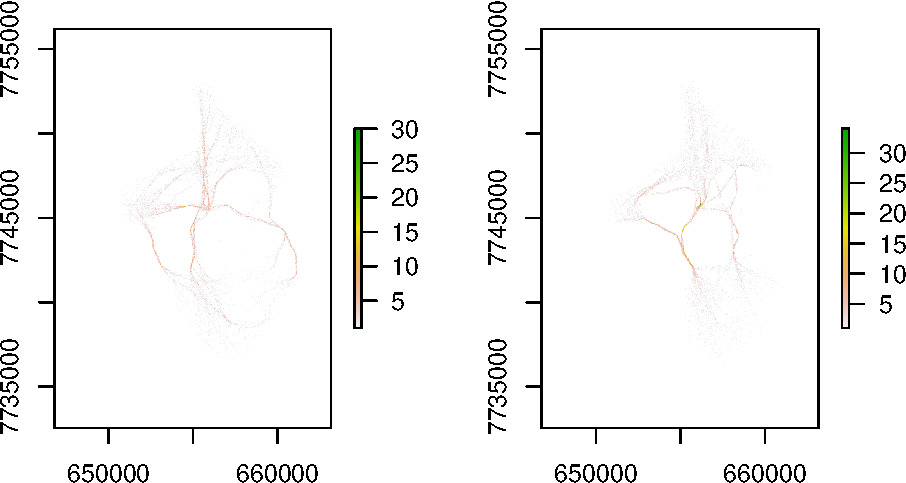
\includegraphics{understanding_resistance_values_files/figure-latex/unnamed-chunk-3-1} \end{center}

\begin{center}\includegraphics{understanding_resistance_values_files/figure-latex/unnamed-chunk-3-2} \end{center}

\begin{center}\includegraphics{understanding_resistance_values_files/figure-latex/unnamed-chunk-3-3} \end{center}

\begin{center}\includegraphics{understanding_resistance_values_files/figure-latex/unnamed-chunk-3-4} \end{center}

\begin{center}\includegraphics{understanding_resistance_values_files/figure-latex/unnamed-chunk-3-5} \end{center}

\begin{Shaded}
\begin{Highlighting}[]
\CommentTok{# proportional change}
\NormalTok{prop.change <-}\StringTok{ }\ControlFlowTok{function}\NormalTok{(before, after) }\DecValTok{100} \OperatorTok{*}\StringTok{ }\NormalTok{(after}\OperatorTok{/}\NormalTok{before }\OperatorTok{-}\StringTok{ }\DecValTok{1}\NormalTok{)}

\NormalTok{mat.prop.change <-}\StringTok{ }\KeywordTok{mapply}\NormalTok{(prop.change, mat.lu.std, mat.lu.zon.std, }\DataTypeTok{SIMPLIFY =}\NormalTok{ F)}

\CommentTok{# plot}
\KeywordTok{mapply}\NormalTok{(img, mat.prop.change, sp)}
\end{Highlighting}
\end{Shaded}

\begin{center}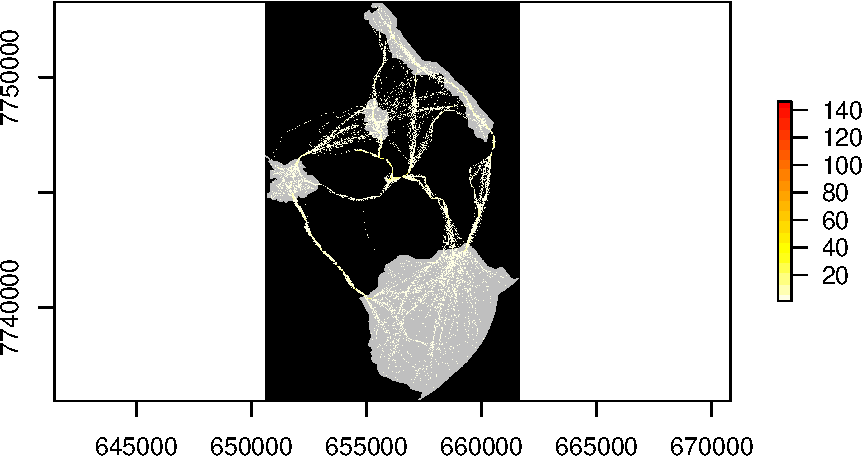
\includegraphics{understanding_resistance_values_files/figure-latex/unnamed-chunk-4-1} \end{center}

\begin{center}\includegraphics{understanding_resistance_values_files/figure-latex/unnamed-chunk-4-2} \end{center}

\begin{center}\includegraphics{understanding_resistance_values_files/figure-latex/unnamed-chunk-4-3} \end{center}

\begin{center}\includegraphics{understanding_resistance_values_files/figure-latex/unnamed-chunk-4-4} \end{center}

\begin{center}\includegraphics{understanding_resistance_values_files/figure-latex/unnamed-chunk-4-5} \end{center}


\end{document}
